\documentclass{article}

\usepackage{fancyhdr}
\usepackage{graphicx}
\usepackage{ragged2e}
\usepackage{hyphenat}
\usepackage[margin=1.25in]{geometry}
\usepackage{xcolor}


\graphicspath{{./../imgs/}}

\pagestyle{fancy}
\fancyhf{}

\fancyhead[L]{\color{lightgray}{\tiny ODIN Drone Concept of Operations (ConOps)}}
\fancyhead[R]{\color{lightgray}{\nouppercase{\tiny \leftmark}}}
\fancyfoot[C]{\thepage}

\begin{document}

\begin{titlepage}
    \begin{figure}
        \centering
        
\includegraphics[scale=1.25]{Bifrost_Logo.png}
    \end{figure}

    \vspace*{1cm}
    \justifying

    {\noindent\huge \textbf{\nohyphens{ODIN Drone Concept of \\ Operations (ConOps)}} \\}
    {\noindent\large \textbf{Version 1.0} \\}

    \vfill

    {\noindent\large \textbf{Prepared by:} \\}
    {\noindent\large \textbf{Bifrost Space Systems}}
\end{titlepage}

\tableofcontents
\newpage

\section{Summary/Mission Concept}
\vspace{0.5cm}

\begin{figure}[h]
    \centering
    \caption{ODIN Drone Mission Phases}
    \label{fig:ConOps_Graphic}
    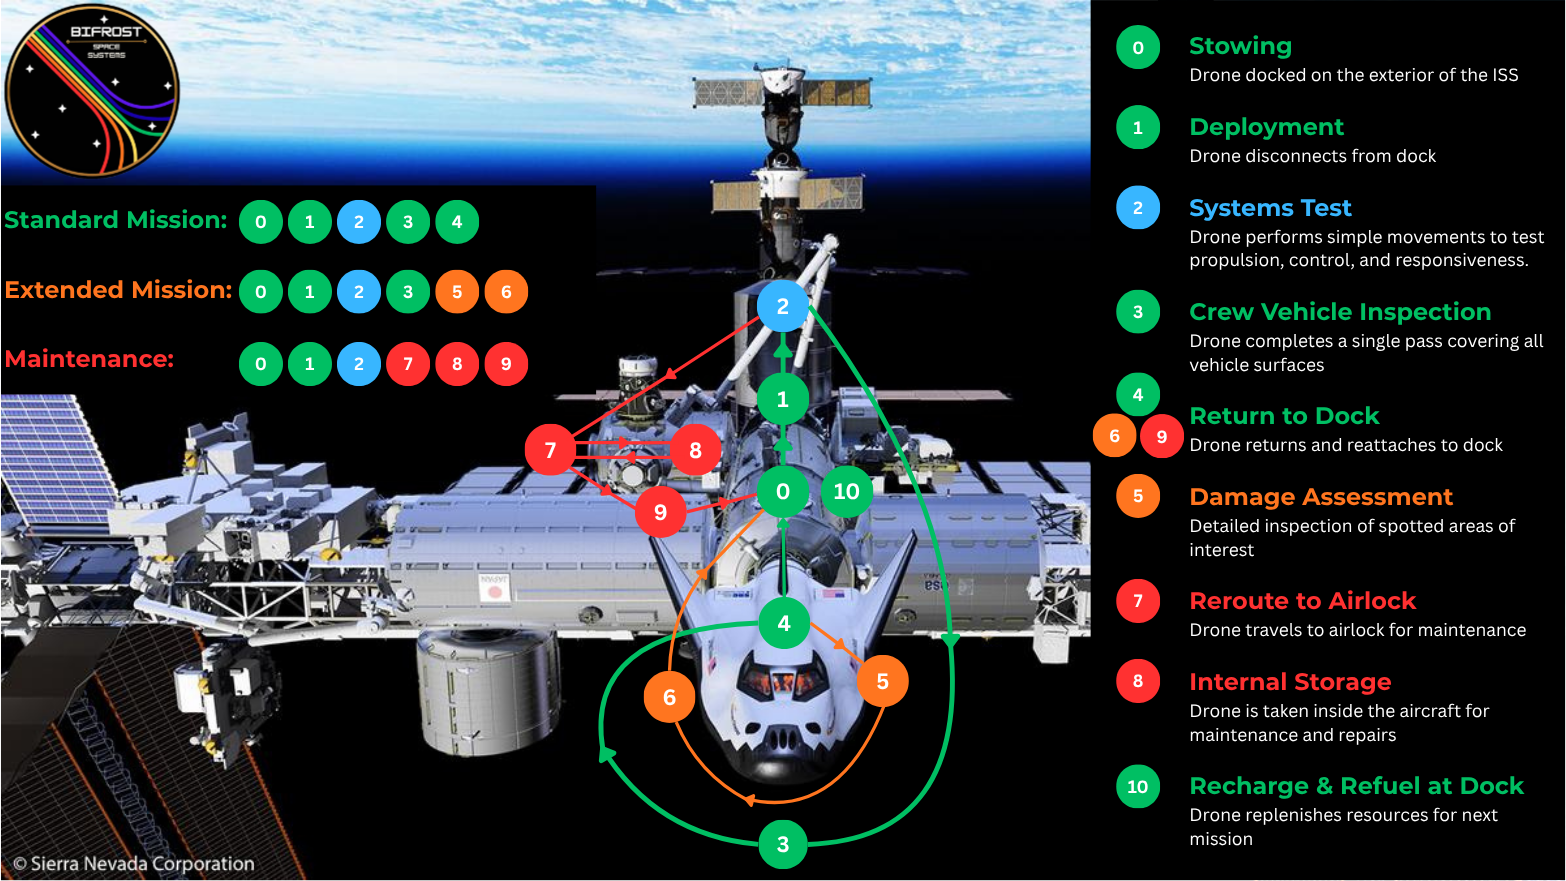
\includegraphics[width=\textwidth, keepaspectratio]{ConOps_Graphic.png}
\end{figure}

\vspace{0.5cm}
\noindent The ODIN drone will ensure the safety of all spacecraft returning to Earth from the ISS. 
Integrating its systems with the ISS, the drone will conduct a scan of spacecraft. 
It will use a camera to analyze the surface of approaching spacecraft, searching for any and all surface damages that may have been accrued during launch.

\newpage

\section{Mission Phases}
The following sections describe the mission phases of the ODIN drone.

\subsection{Stowage/Pre-Use}
Initially turned off, conduct inspection (leaks, damage), (install fuel tank(s) and batter(ies) if stored separately), turn on, pre-flight checks.

\subsection{Flight Phase}
\subsubsection{Systems Test}
During all flight phases of ODIN, the first operation completed after undocking is a flight systems test. 
This test ensures that the control and propulsion systems are operating nominally. 
If anomalies are detected, the mission is re-routed, and the operations of \ref{subsubsec:Maintenance} are followed.

\subsubsection{Nominal Operations}
Following the systems test, ODIN progresses on its mission plan. 
The drone is navigated to the crew vehicle where a standard inspection of the vehicle is completed. 
If the first pass inspection is determined to be sufficient, the ODIN operators move on to \ref{subsubsec:Return}, else, \ref{subsubsec:Anomaly_Inspection} is followed. 

\subsubsection{Anomaly Inspection}
\label{subsubsec:Anomaly_Inspection}
If an anomaly is detected, the ODIN crew will return to the location of the anomaly to re-inspect this section. 
Once enough data is collected to determine the proper course of action for the crew vehicle, operators move to \ref{subsubsec:Return}. 

\subsubsection{Return}
\label{subsubsec:Return}
ODIN is piloted back to its stowage area where it is re-docked to the station. 

\subsubsection{Maintenance}
\label{subsubsec:Maintenance}
If an anomaly is detected in ODIN's systems, then the drone will be brought into the station for maintenance. 
If the anomalies are not critical for flight controls, ODIN can be piloted to an airlock for retrieval. 
If an anomaly is detected that is critical for flight control, case specific procedures will need to be followed to retrieve the drone and to ensure the safety of the crew and to protect the space station from damage. 
Once the drone is retrieved and brought into the station, repairs can be made to restore functionality to the ODIN drone.
Once ODIN's functionality is restored, the drone can then be returned to its dock where nominal operations can once again be conducted.

\subsection{Post-Use/Storage}
After a mission has been completed and ODIN has returned to its dock, a post-mission inspection is completed. 
After the inspection is complete, ODIN is powered off until next usage. 

\newpage
\section{Sub-System Overview}
\subsection{Structures}
blah

\subsection{Materials}
blah

\subsection{Propulsion}
blah

\subsection{Controls}
blah

\subsection{Power}
blah

\subsection{Communications/Command}
The communication/command system will facilitate the astronauts' interactions with the ODIN drone. 
The system will utilize a radar system (TBD) to track ODIN's position and velocity. 
The communication/command system will also utilize a TBD camera for inspection in addition to providing a live feed for piloting ODIN.  
The communication/command system will have a radio control unit to allow the user to pilot ODIN and conduct vehicle inspection. 

\newpage
\section{References}

\end{document}